% !TEX root = ../main.tex

\chapter{Automated Adaptive Design}
\label{chp:design}

From tuning microscopes to designing surveys on politics, all problems of 
experimental design can be reduced to the same mathematical abstraction:
choosing a design that maximizes the expected information gained from the 
experiment.
Bayesian experimental design (BED)~\citep{chaloner1995bayesian,sebastiani2000maximum} 
provides a powerful framework for this abstraction.  In BED
one constructs a likelihood model for the experiment outcome and then uses this, along
with a prior on the parameters one wishes to learn about, to find the experimental setup
that maximizes the expected information gathered by the experiment.  
If the model is correct, this forms a design strategy that is optimal from
an information-theoretic viewpoint \citep{sebastiani2000maximum}.  
The general nature of its formulation means that BED can, at least in principle, be applied
to almost any experimental design situation and it has been successfully used in a wide
array of fields such as psychology~\citep{myung2013tutorial,Cavagnaro:discounting,vincent2017darc},
Bayesian optimization~\citep{hennig2012entropy,hernandez2014predictive}, and
bioinformatics~\citep{vanlier2012bayesian}. \Bad can be particularly useful in \emph{sequential}
design settings, where it provides a means of constructing adaptive strategies that use
previous experience in order to make decisions which optimize the sequential learning process.

Unfortunately, as we alluded to in the previous chapter, BED problems, in
general,  require the calculation of a nested estimation.
In this chapter we will provide a brief introduction to BED and show how our results
from the last chapter can be used to derive a new estimator for BED equations 
which has a better convergence rate for discrete output problems than the na\"{i}ve
estimator often used.  We will further introduce a novel framework for automating the
design of sequential experiments and demonstrate how this can be
effectively applied to automating psychological trials~\citep{vincent2017darc}.  

% !TEX root = ../main.tex

\section{Bayesian Experimental Design}
\label{sec:design:bed}

In this section we will introduce the BED equations more formally.
Let the parameters of interest be denoted by $\theta \in \Theta$ for which we define a prior distribution $p(\theta)$.
Let the probability of achieving outcome $y\in\mathcal{Y}$, given parameters $\theta$ 
and a design $d \in \mathcal{D}$, be defined by likelihood model $p(y | \theta, d)$.
Under our model, the outcome of the experiment given a chosen $d$ is distributed according to
\begin{equation}
\label{eq:marginal_def}
p(y | d) = \int_{\Theta} p(y,\theta | d) d\theta = \int_{\Theta} p(y | \theta, d) p(\theta) d\theta.
\end{equation}
where we have used the fact that $p(\theta)=p(\theta|d)$ because $\theta$ is independent of the design.
Our aim is to choose the optimal design $d$ under some criterion. 
We, therefore, define a utility function, $U(y,d)$, representing the utility of choosing a design $d$ 
and getting a response $y$.
Typically our aim is to maximize information gathered from the experiment, and so we set 
$U(y,d)$ to be the gain in Shannon information between the prior and the posterior:
\begin{align}
\label{eq:shannon_inf}
U(y,d) &= \int_{\Theta} p(\theta |y, d) \log(p(\theta |y, d)) d\theta -\int_{\Theta} p(\theta) \log(p(\theta))d\theta
\end{align}
However, we are still uncertain about the outcome. Thus, we use the expectation of $U(y,d)$ with respect to $p(y | d)$
as our target:
\begin{align}
\bar{U}(d) 
&=\int_{\mathcal{Y}} p(y|d) \left(
\int_{\Theta} p(\theta | y, d)\log(p(\theta |y, d)) d\theta - 
\int_{\Theta} p(\theta) \log(p(\theta)) d\theta \right) dy \nonumber\\
&=\int_{\mathcal{Y}}\int_{\Theta} p(y,\theta | d)\log\left(\frac{p(\theta |y, d)}{p(\theta)}\right)d\theta dy. 
\label{eq:u_bar_1}
\end{align}
noting that this corresponds to the mutual information between the parameters $\theta$ and
the observations $y$.  The Bayesian-optimal design is then given by
\begin{equation}
\label{eq:d_star}
d^* = \argmax_{d \in \mathcal{D}} \bar{U}(d).
\end{equation}

We can intuitively interpret $d^*$ as being the design that most reduces the uncertainty in $\theta$
on average over possible experimental results.  If our likelihood model is correct, i.e. if experimental outcomes
are truly distributed according to $p(y | \theta, d)$ for a given $\theta$ and $d$, then it is easy to see 
from the above definition that
$d^*$ is the true optimal design, in terms of information gain, given our current information about
the parameters $p\left(\theta \right)$.  

In practice, our likelihood model is an approximation of
human behaviour, while the fact that we have a series of design problems will also change the
relative optimality of each design (see Section~\ref{sec:design:seq}).  The former is unavoidable due
to the obvious fact that it is impossible to construct a perfect model for human behaviour.  The latter
can at least in theory be mitigated by incorporating the effect of future possible designs on the
current design (see for example~\cite{gonzalez2016glasses}), but in practice this will generally be
intractable as it requires multiple levels of estimation nesting with the associated problematic convergence
rates shown in Chapter~\ref{chp:nest}. 

Despite these approximations, myopic Bayesian experimental design remains a very powerful and
statistically principled approach that is typically significantly superior to other, more heuristic based,
alternatives.  For example, the state-of-the-art entropy based Bayesian optimization acquisition strategies we 
discussed in Section~\ref{sec:opt:BO:acq:inf} are particular cases of BED.
The main draw back to the Bayesian experimental design 
approach is, in fact, that it is typically difficult and computationally intensive to carry out.  
Not only does it represent an optimisation 
of an intractable expectation, this expectation is itself a nested estimation because
the integrand is itself intractable (due to the $p\left(\theta | y, d\right)$ term).
% !TEX root =  main.tex

\section{An Improved Estimator for Discrete Problems}
\label{sec:bo-design}

As we explained in the last section, estimating $d^*$ is in general challenging
because the posterior $p(\theta |y, d)$ is rarely known in closed form.  
One popular method within the psychology literature is to use a grid-search approach 
to the required inference~\citep{PSImethod:1999, Prins:2013gr}, 
which subsequently provides (biased) estimates for $p(\theta |y, d)$.
However, this is highly unsatisfactory for a host of obvious reasons such as the generally
poor performance of grid-search for inference, the use of a nested estimation procedure
with accompanying poor performance as shown in Chapter~\ref{chp:nest}, and the need to carefully
choose the grid.

To address these issues, we instead derive a nested Monte Carlo estimator as per, for example,
\cite{myung2013tutorial} and further
show how, when $y$ can only take a finite number of values,
a substantially improved, non-nested, Monte Carlo estimator can be derived using the
results from Chapter~\ref{chp:nest}.
The first step is to rearrange~\eqref{eq:u_bar_1} using Bayes' rule (remembering
$p(\theta)=p(\theta|d)$)
\begin{align}
\label{eq:u_bar_2}
\begin{split}
\bar{U}(d)
=& \int_{\mathcal{Y}}\int_{\Theta} p(y,\theta | d) \log\left(\frac{p(y | \theta, d)}{p(y |d)}\right) d\theta dy \\
=&\int_{\mathcal{Y}}\int_{\Theta} p(y,\theta | d) \log(p(y | \theta, d)) d\theta dy - \int_{\mathcal{Y}} p(y | d) \log(p(y | d))dy.
\end{split}
\end{align}
The former term can now be evaluated using standard MC approaches as the integrand is analytic,
namely we can use
\begin{align}
\bar{U}_1(d) = &\int_{\mathcal{Y}}\int_{\Theta} p(y,\theta | d) \log(p(y | \theta, d)) d\theta dy
\approx \frac{1}{N} \sum_{n=1}^{N} \log(p(y_n | \theta_n, d)) \label{eq:U1_MC}
\end{align}
where $\theta_n \sim p(\theta)$ and $y_n \sim p(y|\theta=\theta_n, d)$.\footnote{Note 
	that evaluating~\eqref{eq:U1_MC} involves both
sampling from $p(y | \theta, d)$ and directly evaluating it point-wise.
The latter of these cannot easily be avoided, but in the scenario where we
do not have direct access to a sampler for $p(y | \theta, d)$, we can
use the standard importance sampling trick, sampling instead
$y_n \sim q(y|\theta=\theta_n, d)$ and weighting the samples in~\eqref{eq:U1_MC}
by $w_n = \frac{p(y_n|\theta_n, d)}{q(y_n|\theta_n, d)}$.}
In contrast, the second term of~\eqref{eq:u_bar_2} is not directly amenable to standard MC estimation
as the marginal $p(y|d)$ represents an expectation
and taking its logarithm represents a nonlinear functional mapping.  
Here we have
\begin{align}
\bar{U}_2(d) = &\int_{\mathcal{Y}} p(y | d) \log(p(y | d))dy
\approx \frac{1}{N} \sum_{n=1}^{N} \log \left(\frac{1}{M} \sum_{m=1}^{M} p(y_n | \theta_{n,m}, d)\right) \label{eq:U2_MC}
\end{align}
where $\theta_{n,m} \sim p(\theta)$ and $y_n \sim p(y | d)$.  We can sample the latter by first sampling an otherwise unused $\theta_{n,0} \sim p(\theta)$ and 
then sampling a single corresponding $y_n \sim p(y | \theta_{n,0}, d)$.

Putting~\eqref{eq:U1_MC} and~\eqref{eq:U2_MC} together (and renaming
$\theta_n$ from~\eqref{eq:U1_MC} as $\theta_{n,0}$ for notational
consistency with ~\eqref{eq:U2_MC})  we now have the following complete estimator,
implicitly used by \cite{myung2013tutorial} amongst others,
\begin{align}
\label{eq:exp-des-nmc}
\bar{U}(d) 
& \approx  
\frac{1}{N} \sum_{n=1}^{N} \left[ \log(p(y_n | \theta_{n,0},d)) 
- \log \left(\frac{1}{M} \sum_{m=1}^{M}p(y_n | \theta_{n,m},d)\right) \right]
\end{align}
where $\theta_{n,m} \sim p(\theta) \; \forall m \in 0:M, \;n \in 1:N$ and $y_n \sim p(y|\theta=\theta_{n,0}, d) \; \forall n \in 1:N$.
This na\"{i}ve NMC estimator, Anglican code for which is provided in 
Figure~\ref{fig:nest:exp}, gives a convergence
rate of $O(1/N+1/M^2)$ as per Theorem~\ref{the:Repeat}.

We now show that if $y$ can only take on one of $C$ possible values ($y_1, \ldots, y_C$), 
we can achieve significant improvements in the convergence rate by using a similar approach to that
introduced in Section~\ref{sec:app:finite-res} to derive the following non-nested estimator for~\eqref{eq:u_bar_2}
\begin{align}
&\bar{U}(d)=\int_{\mathcal{Y}}\int_{\Theta} p(y,\theta | d) \log(p(y | \theta, d)) d\theta dy - \int_{\mathcal{Y}} p(y | d) \log(p(y | d))dy 
\nonumber \\
&= \int_{\Theta} \left[\sum_{c=1}^{C} p(\theta) p(y_c|\theta, d) \log(p(y_c | \theta, d)) \right] d\theta
-\sum_{c=1}^{C} p(y_c | d)\log(p(y_c | d))  \nonumber \\
&\approx 
\frac{1}{N} \sum_{n=1}^{N} \sum_{c=1}^{C} p(y_c | \theta_n, d) \log\left(p(y_c | \theta_n, d)\right)
- \sum_{c=1}^{C} \left[\left(\frac{1}{N}\sum_{n=1}^{N} p(y_c | \theta_n, d)\right) \log \left(\frac{1}{N} \sum_{n=1}^{N} p(y_c | \theta_n, d)\right) \right] \label{eq:u_bar_MC}
\end{align}
where $\theta_n \sim p(\theta) \; \forall n \in 1,\dots,N$ and $y_c$ are fixed constants.
Here our estimate is a deterministic function of a number of separate Monte Carlo estimators.  
Because there is no trivial canceling of terms and there are no issues with continuity of the
function because $x\log(x)=0$, and each $p(y_c | \theta_n, d)\le1$,
no complications originate from this function application and the MSE of our estimator will
converge at the standard MC error rate of $O(1/N)$. This requires $T=O(NC)$ calculations and
so we can express the per evaluation convergence rate as $O(C/T)$.  This compares to 
an optimal rate of $O(1/T^{2/3})$ for~\eqref{eq:exp-des-nmc}.  Though relatively straightforward,
to the best of our knowledge, this superior estimator has not appeared in the literature prior
to our own work~\citep{rainforth2017pitfalls,vincent2017darc}.

% !TEX root =  main.tex

\section{Automating Sequential Design Problems}
\label{sec:design:seq}

We have thus far assumed that there is no previous data (i.e. design-outcome pairs).
Though this static experimental design setup is of use in its own right, the real potential
of \Bad is not realized until one considers using it in \emph{sequential} settings.
Here \Bad provides a framework for adaptively making an optimal series of decisions
in an online fashion in the presence of uncertainty.  For example, imagine a psychology
trial where we ask a participant a series of questions to learn about certain behavior
characteristics.  If a human is conducting this experiment they are likely to adapt
the questions they ask as they learn about the participant to try and maximize the information
gathered.  Similarly, a detective conducting an investigation will
adapt the questions they ask about a suspect as they learn information from previous
answers.  Sequential \Bad provides a mathematical framework for reasoning about and optimizing
such processes, thereby providing a means of developing effective machine learning systems to
carry out such tasks.
  It is quite incredibly general and can, at least in theory, be applied to any
situation where we aim to sequentially gather information.  For example, in Section~\ref{sec:opt:BO:acq:inf}
we described strategies for Bayesian optimization which explicitly use the \Bad equations
to sequentially gather information about the location of the optimum.  One could envisage similarly
using the framework for conducting proposal adaptation for inference problems.  We could
use it in vision tasks to prioritize where to look in a scene.  The number of potential
applications is endless.

From a mathematical perspective, we can generalize to the sequential design setting by 
incorporating data in the standard Bayesian fashion such that
at experiment iteration $t$, we replace $p\left(\theta\right)$ with 
$p\left(\theta | d_{1:t-1}, y_{1:t-1}\right)$, where $d_{1:t-1}$ and  $y_{1:t-1}$ are 
respectively the designs and outcomes at previous iterations.
The likelihood $p\left(y_t | \theta, d_t\right)$, on the other hand, is unchanged (presuming it 
is a parametric distribution) as, conditioned on 
$\theta$ and $d$, the current outcome is independent of the previous data.
Putting this together, we get that the expected information gain criteria for the
sequential case is
\begin{align}
\label{eq:u_bar_seq}
\begin{split}
\bar{U}_t(d)
=&\int_{\mathcal{Y}}\int_{\Theta} p\left(\theta | d_{1:t-1}, y_{1:t-1}\right)
p(y_t | \theta, d_t) \log(p(y_t | \theta, d_t)) d\theta dy_t \\
&- \int_{\mathcal{Y}} p(y_t | y_{1:t-1}, d_{1:t}) \log(p(y_t | y_{1:t-1}, d_{1:t}))dy_t.
\end{split}
\end{align}
We can now see that these terms are the same as in the non-sequential case,
except that expectations are taken with respect to $p\left(\theta | d_{1:t-1}, y_{1:t-1}\right)$
rather than $p(\theta)$.  Therefore, we can use the same Monte Carlo estimators
\eqref{eq:exp-des-nmc} and \eqref{eq:u_bar_MC}, but instead drawing $\theta_n\sim p\left(\theta | d_{1:t-1}, y_{1:t-1}\right)$.

In the rest of this section, we will outline a framework for automating such sequential
adaptive design problems.  This takes on a somewhat probabilistic programming flavor, as
the aim is to develop a system where the user provides only information about the model and
design space, with the next chosen design calculated automatically when provided with
the outcome of the last.  However, as we will discuss in Section~\ref{sec:disc:design}, this actually goes
beyond the capabilities of current PPS.  What we present is by no means a complete solution to
this problem and certainly does not represent a PPS itself, but it does perhaps provide an important
step towards building such a hypothetical system.   Indeed the framework has already been
applied to provide automated sequential BED for a very restricted model class existing in the form of
the DARC toolbox~\citep{vincent2017darc} introduced in Section~\ref{sec:design:darc}.

\subsection{Parameter Inference}
\label{sec:design:auto:inf}

Unlike $p\left(\theta\right)$, it is typically not possible to evaluate, or sample from, $p\left(\theta | d_{1:t-1}, y_{1:t-1}\right)$ exactly -- we need to perform Bayesian inference to estimate it.  Noting
the implicit assumption of the likelihood model that observations are independent of one other given the
parameters we have
\begin{align}
p\left(\theta | d_{1:t-1}, y_{1:t-1}\right) \propto p(\theta) \prod_{i=1}^{t-1} p(y_i | \theta, d_i)
\end{align}
which is a typical Bayesian inference problem, such that we can use Monte Carlo inference
to generate the required samples $\theta_n$.  Note that this setup is very general.   For example, there might
be a term in $\theta$ for each round of the experiment, leading to a non-Markovian state space model as
per Section~\ref{sec:part:smc:nmssm}.
There are many suitable candidates for the required inference such as those discussed in Chapters~\ref{chp:inf} and
\ref{chp:part}.
The relative merit of these will depend on
characteristics of the problem such as multi-modality, the dimensionality of $\theta$, and the total
number of questions that will be asked.  For the DARC toolbox introduced later we will use 
population Monte Carlo (PMC) \citep{cappe2004population}.  However, our contribution here is independent of
the choice of inference algorithm, provided that algorithm can be appropriately automated for the range
of problems one wishes to run, as is the case for a PPS.  One salient feature of note though is
that, by its nature, the inference problem requires a series of targets to be approximated and so
inference methods that can effectively exploit the approximation of the previous target (such as particle-based methods, see
 Chapter~\ref{chp:part}) are likely to be particularly effective.

\subsection{Design Optimization}
\label{sec:design:auto:optimization}

We have now derived an estimator for $\bar{U}_t(d)$ and demonstrated how we can generate the
samples required to evaluate this estimator.  We will now look at how to optimize for $d$.  
Our problem requires the optimization of an intractable expectation and thus shares substantial
similarity to the problems considered in Chapter~\ref{chp:bopp}.  Indeed BOPP could form a suitable
approach to estimating $d^*$ at each iteration for many problems.  However, BOPP is a somewhat heavy
duty estimation algorithm that may not be suitable for problems that are relatively simple,
but for which speed is paramount.  Many of the possible applications of our approach, such
as the DARC toolbox, require rerunning in real-time with human participants, for which BOPP would
thus be inappropriate.\footnote{Nonetheless, if the surrogate in BOPP
	was replaced with a more lightweight regressor, e.g. a random forest~\cite{hutter2011sequential},
	then the resulting algorithm could prove a viable alternative even under strict time pressure.}
We instead construct a new approach
that exploits the fact that~\eqref{eq:u_bar_MC} need not generate distinct $\theta_n$ to evaluate
different designs.  Our novel method combines ideas from both the bandit and
Monte Carlo literatures~\citep{amzal2006bayesian,neufeld2014adaptive} by adaptively 
allocating resources to a set of candidate designs.  We will presume that there are some fixed number 
of candidate designs $\mathcal{D} = \{d_k\}_{k=1:K}$ which could be randomly (or quasi-randomly)
sampled up front if the design space is continuous.  This assumption is made because the 
algorithm was designed with a particular application in mind, namely the DARC toolbox for which $K$
is generally not more than a few thousand.  We note, though, that it should be possible to relax this
assumption by incorporating MCMC transitions in a manner akin to~\citep{amzal2006bayesian}.

The underlying idea of the approach is that we are willing to accept higher variance in the integral estimates for lower utility designs as this error is unlikely to lead to an incorrect estimation of the optimum.
Therefore, we desire to take more Monte Carlo samples, and thus achieve a more accurate estimate, for the designs we estimate to have a higher chance of being the optimal design, given the current noisy estimates.
At a high level, this is similar  to the idea of Thompson sampling
where a candidate is sampled in proportion to its probability of being the best~\citep{thompson1933likelihood}, 
a technique commonly used in the bandit literature~\citep{agrawal2012analysis}.

\begin{algorithm}[t]
	\small
	\captionsetup{labelfont=bf, justification=justified,singlelinecheck=false}
	\caption{Design optimisation \label{alg:des-opt}}
	\setstretch{1.1}
	\begin{algorithmic}[1]
		\renewcommand{\algorithmicrequire}{\textbf{Inputs:}}
		\renewcommand{\algorithmicensure}{\textbf{Outputs:}}				 
		\Require Reservoir $\{\theta_m\}_{m=1:M}$, likelihood $p(y | \theta, d)$,
		candidate designs $\mathcal{D} = \{d_k\}_{k=1:K}$, number of particles $N$, number of steps
		$L$, annealing schedule $\gamma : \mathbb{Z}^+ \rightarrow \mathbb{R}$, minimum selection probability $\rho$
		\Ensure Chosen design $d^*$
		\State $\hat{U}_k \leftarrow 0 \quad \forall k \in \{1,\dots,K\}$ \Comment Initialize estimates
		\State $q_k \leftarrow 1/K \quad \forall k \in \{1,\dots,K\}$ \Comment Initialize selection probability
		\For{$\ell= 1 \colon L$}
		\State $\{n_k\}_{k=1:K} \sim \textsc{Multinomial}(N,\{q_k\}_{k=1:K})$ \label{line:des-opt:sample-nsamples}
		\Comment Sample number of new samples to add\footnotemark
		\For{$k = 1 \colon K$}
		\State $\hat{\theta}_{j} \leftarrow \textsc{Discrete}\left(\left\{\theta_m\right\}_{m=1:M}\right) \quad \forall j=1,\dots,n_k$ \label{line:des-opt:draw-theta}
		\Comment Draw $n_k$ samples from reservoir
		\State $\hat{U}_k \leftarrow \textsc{Update}\left(\hat{U}_k,\{\hat{\theta}_j\}_{j=1:n_k},p(y | \theta, d),d_k\right)$
		\label{line:des-opt:refine-U}
		\Comment Use new samples to refine estimate %for $\hat{U}_k$
		\EndFor	
		\State $\tilde{q}_k \leftarrow \hat{U}_k^{\gamma(\ell+1)} \quad \forall k = 1,\dots,K$ 
		\label{line:des-opt:set-p}
		\Comment Unnormalized selection probability $= \text{annealed} ~\hat{U}_k$
		\State $Z \leftarrow \sum_{k=1}^{K} \tilde{q}_k $ \Comment Normalization constant
		\State $q_k \leftarrow \max\left(\frac{\rho}{N},\frac{\tilde{q}_k }{Z}\right) \quad \forall k = 1,\dots,K$ \Comment Ensure probabilities are all at least minimum value
		\State $q_k \leftarrow \frac{q_k}{\sum_{k=1:K} q_k} \quad \forall k = 1,\dots,K$ 
		\label{line:des-opt:renorm}
		\Comment Renormalize
		\EndFor	
		\State $k^* \leftarrow \argmax_{k \in \{1,\dots,K\}} \hat{U}_k$ \Comment Best design is one with highest $\hat{U}_k$
		\State \Return $d_{k^*}$
	\end{algorithmic}
\end{algorithm}
\footnotetext{One could use systematic ``resampling'' here too 
	as per Section~\ref{sec:inf:foundation:resampling}.}

An overview of our approach is given in Algorithm~\ref{alg:des-opt}.  As this shows, our algorithm uses
a \emph{reservoir} of samples $\{\theta_m\}_{m=1:M}$ instead of drawing samples from 
$p\left(\theta | d_{1:t-1}, y_{1:t-1} \right)$ on-demand.  In short, we draw $M$ samples from the
posterior upfront to create the reservoir, then instead of sampling directly from 
$p\left(\theta | d_{1:t-1}, y_{1:t-1} \right)$ during the design optimization,
we draw a sample from the reservoir.  Careful coding (not shown in the algorithm block) ensures 
that each sample in the reservoir is not used more than once in any particular estimate $\hat{U}_k$, while by using
a reservoir that is larger than the number of samples we will need for any individual estimate, we
ensure that the reservoir itself does not cause any approximation in the posterior (though it can cause correlation
between the $\hat{U}_k$).
The use of a reservoir is a key innovation of our approach as it allows
us to modularize the parameter inference and design optimization problems: the inference algorithm
produces a reservoir as output and the optimizer can then run without having to refer back to the
inference algorithm.

The second key innovation of our approach is that rather than calculating each estimate $\hat{U}_k$ in one go, we
exploit the intermediate information from incomplete evaluations to reallocate computational
resources in a manner that has parallels with SMC, SMC search~\citep{amzal2006bayesian}, annealed
importance sampling~\citep{neal2001annealed}, adaptive Monte Carlo via bandit 
allocation~\citep{neufeld2014adaptive}, and the Hyperband algorithm~\citep{li2016hyperband}.
%\footnote{We
%	note that our approach was independently developed prior to publication of~\cite{li2016hyperband} (the relevant
%	code for the DARC toolbox dates back to 2015), but remained unpublished until~\cite{vincent2017darc}.}
%We emphasise though that our method has important differences
%to these previous approaches and constitutes a new algorithm in its own right.
Imagine that we are considering $K$ designs $\mathcal{D} = \{d_k\}_{k=1:K}$ with a total sample budget $\bar{N}K$
and decide to use the same number of samples, $\bar{N}$, to calculate an estimate $\hat{U}_{k}$ for the 
utility of each design.  
After we have taken say $n$ samples
for each estimate, where $1\le n<\bar{N}$, then we will have a set of intermediate estimates $\hat{U}_{1:K}^n$ for
each utility.  Now remembering that our aim is to establish which design is best (i.e. which $\bar{U}_k$ is largest),
we note that our intermediate estimates convey valuable information -- they show that some designs are more
likely to be optimal than others.
Consequently, sticking to our original plan and using the same number of samples, $\bar{N}-n$, 
to complete our final estimates will
be inefficient as some designs will be highly unlikely to be optimal and therefore it is pointless to
spend a noticeable proportion of our computational budget to carefully refine their estimates.  It is clearly 
more efficient, in terms
of the final optimization problem, to take relatively more samples for the promising designs, so that we can better 
distinguish between their relative utilities, even if this results in very poor estimates for the low utility
designs.  This is the key idea of our approach -- to adaptively change the number of samples used to estimate
the utilities for different designs, based on the probability the design may end up being optimal given its
intermediate estimates.

More specifically, given a total budget of $NL=\bar{N}K$ samples for all our estimates,
then we will carry out $L$ rounds of sampling, where at each round we adaptively allocate $N$ samples
between the different estimators in proportion to how relatively promising their respective designs
appear.  To do this,
we \emph{sample a number of samples} to take for each design at each round in proportion to an annealed version of
its utility estimate (line~\ref{line:des-opt:sample-nsamples} of Algorithm~\ref{alg:des-opt}).  
Namely, if $q_{k,\ell}$ is the probability each sample from our budget is assigned
to design $k$ at round $\ell$ and $\hat{U}_{k,\ell}$ is the corresponding running estimate for the utility
of that design, then we have (line~\ref{line:des-opt:set-p} of Algorithm~\ref{alg:des-opt})
\begin{align}
\label{eq:p_k}
q_{k,\ell} \propto (\hat{U}_{k,\ell})^{\gamma(\ell)}
\end{align}
where $\gamma : \mathbb{Z}^+ \rightarrow \mathbb{R}$ is an annealing function (see next paragraph).  
Thus we will, on average,
add $\mathbb{E}[n_{k,\ell}] = q_{k,\ell}N$ samples of $\theta$ to the estimate for $\bar{U}_k$ at round $\ell$
(lines~\ref{line:des-opt:draw-theta} and~\ref{line:des-opt:refine-U} of Algorithm~\ref{alg:des-opt}).
By storing appropriate running estimates (e.g. for $p(y | d_k)$), the estimates can 
be updated with the $n_k$ new samples from the reservoir
$\{\hat{\theta}_j\}_{j=1:n_k}$ at each round.  This corresponds to the \textsc{Update} function in
Algorithm~\ref{alg:des-opt}.

The purpose of the annealing function is to control how aggressive our algorithm is in its allocation of
computational resources to promising designs.
At the early rounds, we are quite uncertain about the relative
utilities and therefore wish to allocate samples fairly evenly.  At the later rounds, we become more certain
about the estimates so we become more aggressive about concentrating our efforts on promising designs.
Therefore $\gamma(\ell)$ is set to increase with $\ell$.

We finish the subsection by noting a small, but important, subtlety of our method.  As introduced so far, our algorithm
is not guaranteed to converge.  For example, it might be that $\hat{U}_{k^*} =0$ after the first round
of sampling where $k^*$ indicates the true optimal design and $\bar{U}_{k^*} \ne0$.  
Presuming that another design has a non-zero estimate at this point, sampling na\"{i}vely from~\eqref{eq:p_k} would 
mean that no additional samples are ever added to $\hat{U}_{k_*}$, even if infinite rounds are undertaken,
meaning that the true optimum will be missed.  To guard against this, we introduce a new parameter $0<\rho\le1$, 
with lines~\ref{line:des-opt:set-p} to~\ref{line:des-opt:renorm} in Algorithm~\ref{alg:des-opt}
ensuring that each $q_{k,\ell}>\frac{\rho}{2N}$ (see~\cite{vincent2017darc}), which in turn ensures that  
$\mathbb{E}\left[\sum_{\ell=1}^{L} n_{k,\ell}\right] >\rho L/2$.
Therefore, for any finite value of $\rho$, each
estimate will, in expectation, be assigned infinitely many samples as $L\rightarrow\infty$, regardless
of the true utilities and the values of $\gamma(\ell)$.\footnote{Note that one should, if desired, be able to instead 
	use an upper confidence bounding strategy~\citep{auer2002using} to produce a zero-regret 
	strategy whilst maintaining convergence}
As we show in the next section, we can
use this to prove the convergence of the algorithm, in the sense of guaranteeing the optimal design
will be found given infinite computational budget.

\subsection{Tying it All Together}
\label{sec:tying-together}

In the previous sections, we have shown how to construct an appropriate target for our design optimization,
estimate this target for a particular design given samples from the posterior on parameters,
produce the required approximate samples for this posterior, and use these samples to find the optimal design.
Algorithm~\ref{alg:bad} shows how these components fit together to produce a framework for
automated online sequential design optimization.  Algorithm parameters have been omitted
for clarity, but we note that it should, in general, be possible to set these to default values if required, e.g. using
the general purpose inference strategies taken by PPSs.
%The algorithm iterates between selecting the optimal design,
%running the experiment, and incorporating the results of the experiment to update the posterior on the
%parameters.  As we have previously explained, our design optimization can be run using a reservoir of
%samples from the posterior, allowing this modularization of the inference and optimization processes.
We finish with the following theoretical result that
shows that the method is guaranteed to return the optimal design at each iteration in the limit of large
computational resources.
\begin{algorithm}[t]
	\small
	\captionsetup{labelfont=bf, justification=justified,singlelinecheck=false}
	\caption{Sequential \Bad \label{alg:bad}}
	\setstretch{1.1}
	\begin{algorithmic}[1]
		\renewcommand{\algorithmicrequire}{\textbf{Inputs:}}
		\renewcommand{\algorithmicensure}{\textbf{Outputs:}}				 
		\Require Prior $p(\theta)$, likelihood $p(y | \theta, d)$, number of experiment iterations $T$,
		candidate designs $\mathcal{D}$
		\Ensure Design-outcome pairs $\{d_t,y_t\}_{t=1:T}$, posterior samples $\{\theta_m\}_{m=1:M}$
		\State $\theta_m\sim p(\theta) \quad \forall m = 1, \dots, M$
		\For{$t=1:T$}
		\State $d_t \leftarrow \textsc{DesignOptimization}\left(\{\theta_m\}_{m=1:M},p(y | \theta, d),
		\mathcal{D}\right)$ \Comment Find next step optimal design
		\State $y_t \leftarrow \textsc{RunExperiment}(d_t)$ \Comment Get outcome using design $d_t$
		\State $\mathcal{D}\leftarrow\mathcal{D}\backslash d_t$ 
		\Comment Eliminate new design from candidate set (optional)
		\State $\{\theta_m\}_{m=1:M} \leftarrow \textsc{Inference}\left(p(\theta),p(y | \theta, d),\{d_i,y_i\}_{i=1:t},
		\{\theta_m\}_{m=1:M} \right)$ 
		\Comment  Update the posterior
		\EndFor
		\State \Return $\{d_t,y_t\}_{t=1:T}$, $\{\theta_m\}_{m=1:M}$
	\end{algorithmic}
\end{algorithm}
\begin{theorem}
	Assume that each $\bar{U}_t$ is a measurable function and 
	that all other requirements for consistency of the chosen inference algorithm are satisfied.\footnote{If the
		chosen inference algorithm also provides almost sure convergence, the result also holds almost surely.}
	Given a finite number of candidate designs $\{d_k\}_{k=1:K}$, fixed parameters $\rho>0$ and $N\in\mathbb{N}^{+}$, and a
	function $\tau : \real \rightarrow \real$ such that $\tau(L)\ge NL \; \forall L$, then using
	Algorithms~\ref{alg:des-opt} and~\ref{alg:bad} to choose design outcome pairs with $M=\tau(L)$
	ensures that the chosen design at each iteration $d_t$ satisfies
	\begin{align}
	\bar{U}_t(d_t)= \max_{d\in\mathcal{D}} \bar{U}_t(d)
	\end{align}
	with high probability in the limit $L\rightarrow\infty$, where 
	$\bar{U}_t(d)$ is defined as per~\eqref{eq:u_bar_seq}.
\end{theorem}
\begin{proof}
	We start by noting that by the definition of $\tau(\cdot)$ then $L\rightarrow\infty$ also predicates
	that $M\rightarrow\infty$ and so by assumption our Monte Carlo estimates made using the output
	of our inference algorithm converge in probability (noting $M\ge NL$ also ensures the reservoir is
	large enough to not need to reuse samples).
	%By~\eqref{eq:nk-bound}, we have $\mathbb{E}\left[\sum_{\ell=1}^{L}  n_{k,\ell}\right]\rightarrow \infty$
	%as $L\rightarrow\infty$ such that the expected number of samples used for each design is infinite. 
	
	As the $n_{k,\ell}$ are not independent, we break each down into two terms
	$n_{k,\ell} = m_{k,\ell}+r_{k,\ell}$ where $m_{k,\ell} \sim \textsc{Binomial}(N,\frac{\rho}{2N})$ and
	$r_{k,\ell} \sim \textsc{Binomial}(N,q_{k,{\ell}}-\frac{\rho}{2N})$ (which induces the appropriate distribution
	on $n_{k,\ell}$).  For any given $k$, all the $m_{k,\ell}$
	are mutually independent and $P(m_{k,\ell} \ge 1) = 1-(1-\frac{\rho}{2N})^N$ ($\rightarrow 1-\exp (-\rho/2)$ 
	as $N\rightarrow\infty$).  Therefore, for any possible $N$ (including $N\rightarrow\infty$) 
	we have $\sum_{\ell=1}^{\infty} P(m_{k,\ell} \ge 1) = \infty$
	and so by the second Borel-Cantelli lemma, the event $m_{k,\ell} \ge 1$ occurs infinitely often with probability $1$.
	Thus, as each $r_{k,\ell}\ge0$, it must also be the case that
	$P(\lim_{L\rightarrow\infty} \sum_{\ell=1}^{L} n_{k,\ell} = \infty) = 1$.
	
	Combining these two results, we have convergence of each of the $K$ estimates $\hat{U}_k$
	at each iteration and so we must choose the optimal design (or one
	the equally best designs if there is a tie)  with high probability in the limit $L\rightarrow\infty$.
\end{proof}
% !TEX root =  main.tex

\section{The DARC Toolbox}
\label{sec:design:darc}

We now demonstrate the utility of our approach by considering its application 
to automating the adaptive design psychology experiments via the DARC (Delay
And Risky Choice) toolbox introduced in~\cite{vincent2017darc}.\footnote{Code available at~ \url{http://github.com/drbenvincent/darc-experiments-matlab}.}  We will only provide
a short introduction here and refer the reader to~\cite{vincent2017darc} for further details.

The DARC toolbox allows users 
to encode their own (or use one of the provided) models for human \emph{discounting} behavior,
whereby psychologists want to learn how delays and uncertainties affect the subjective value people place
on (typically monetary) rewards or costs. Given a model, the toolbox uses the framework from the
previous section to automate in an online fashion 
both the inference of the model parameters and the sequential adaptation of the experiment itself through
choosing the questions the participant is asked.  It, therefore, automates the full run-time experimental 
pipeline  by using the responses from previous questions to perform inference 
and update the internal representation
of the participant and then using this information to ask the most informative questions for a particular
participant as per the BED equations.  The technical innovations introduced earlier is this chapter
are essential in allowing this to be done sufficiently efficiently to permit
real-time usage required for deployment with real participants.

\begin{figure}[t]
	\centering
	\begin{subfigure}[b]{0.49\textwidth}
		\centering
		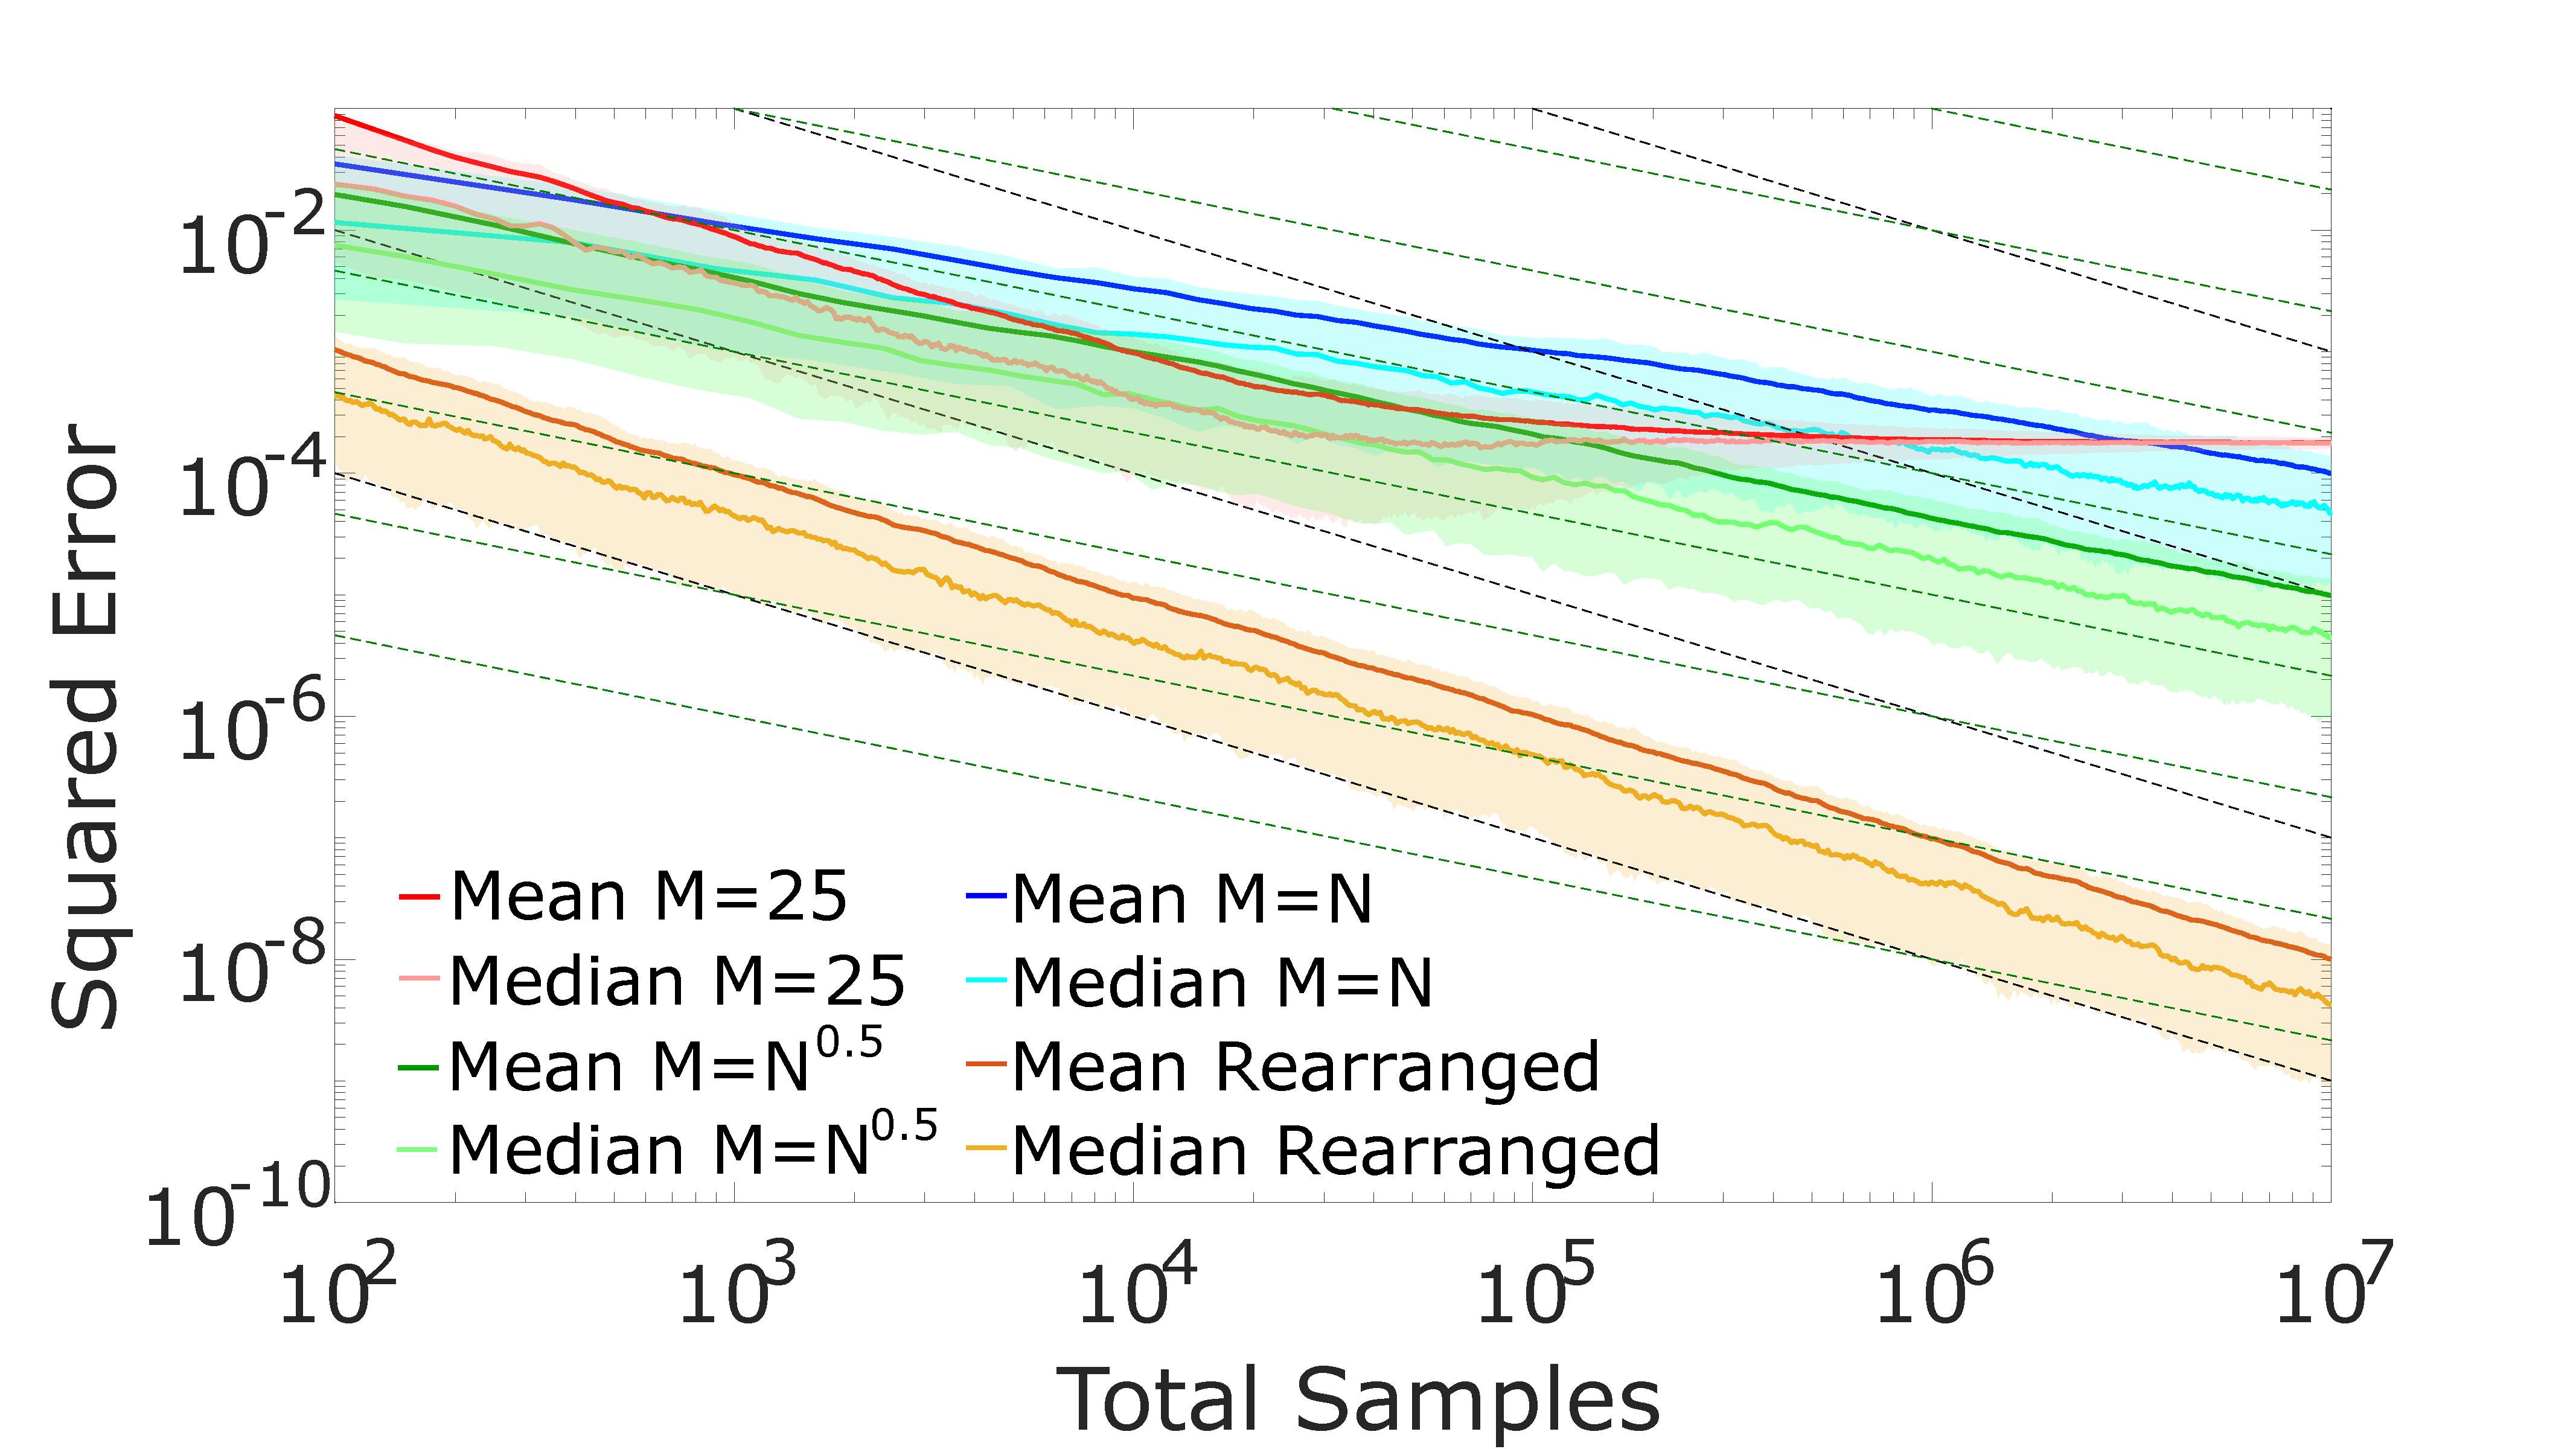
\includegraphics[width=0.99\textwidth,trim={1.5cm 0 3.5cm 0},clip]{exp_conv2}
		\caption{Convergence of BED\label{fig:exp-conv}}
	\end{subfigure}
		\begin{subfigure}[b]{0.49\textwidth}
			\centering
			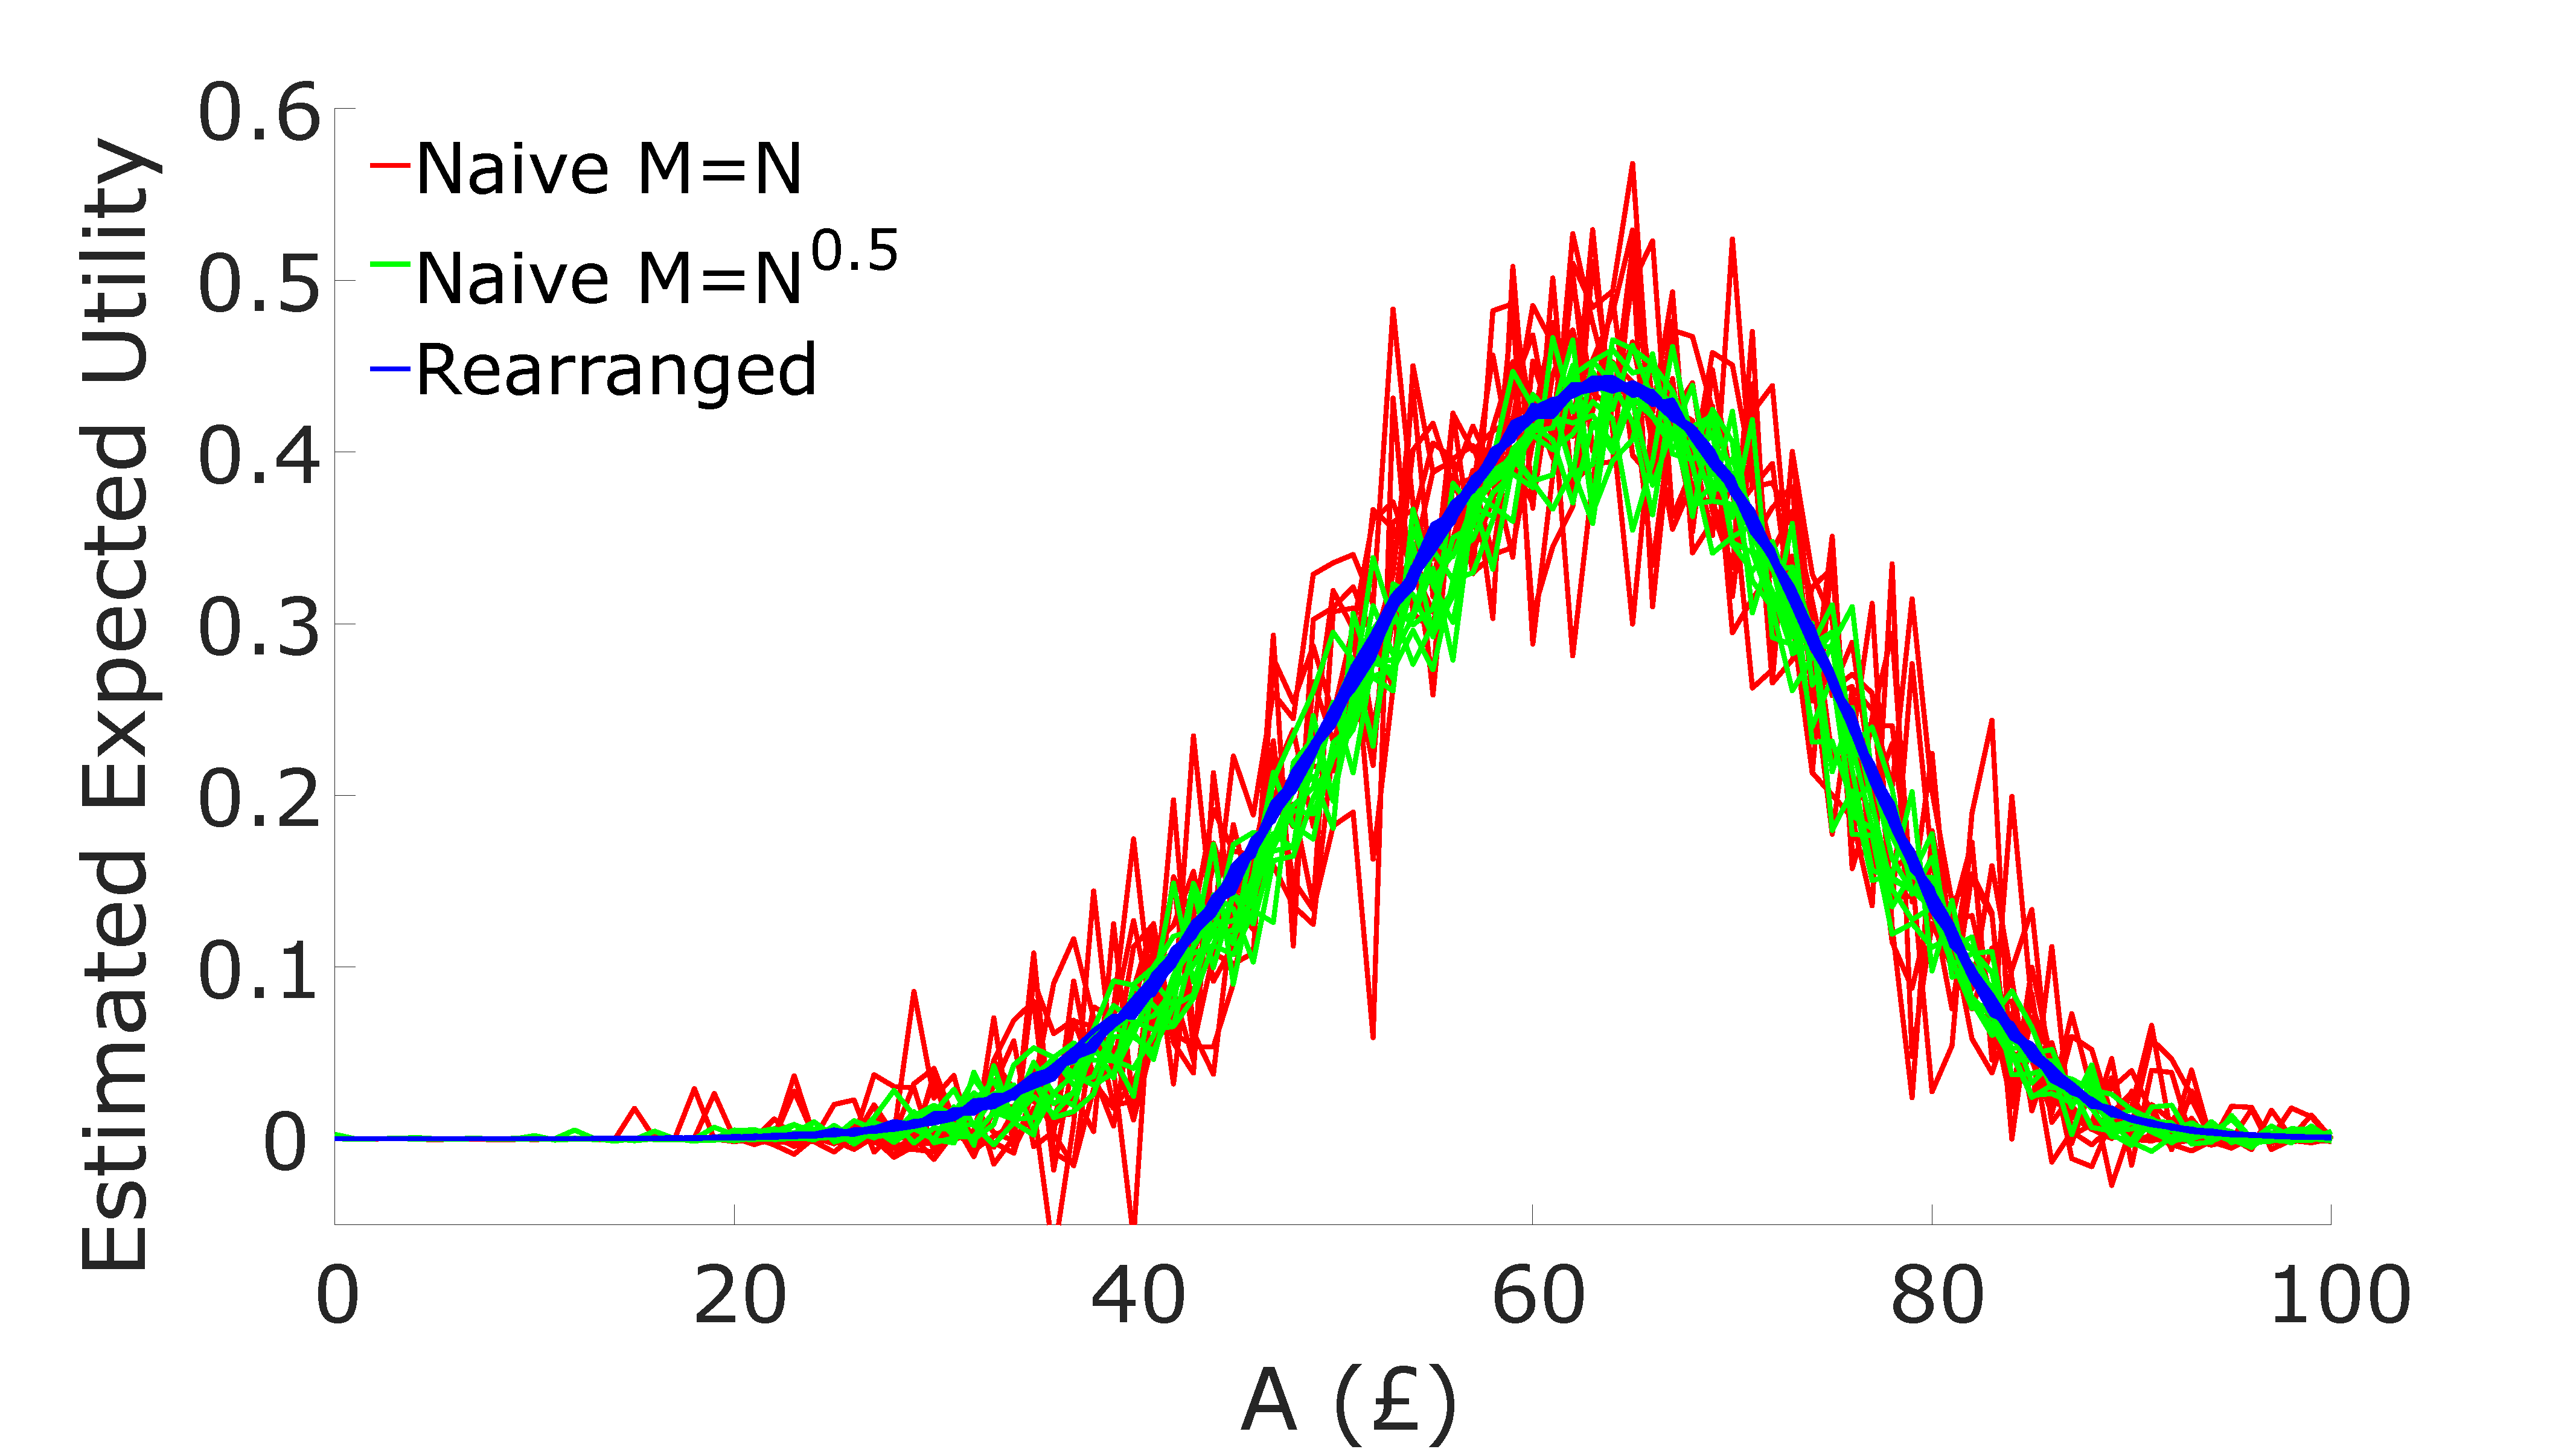
\includegraphics[width=0.99\textwidth,trim={1.5cm 0 3.5cm 0},clip]{dscan_2}
			\caption{Estimated expected utilities \label{fig:exp-d-scan}}
		\end{subfigure}
		\vspace{5pt}
	\caption{(Left) convergence of both NMC and our reformulated
		estimator~\eqref{eq:u_bar_MC} for the BED problem.
		A ground truth estimate was calculated using a single run of the reformulated
		estimator with $10^{10}$ samples.
		Results are averaged over 1000 independent runs, while shaded regions give the 25\%-75\% quantiles. We
		see that the theoretical convergence rates (shown by the dashed lines) are observed in all cases,
		with the advantages of the reformulated estimator particularly pronounced.
		(Right) estimated expected utilities $\bar{U}(d)$for 
		different values of one of the design parameters $A \in \{1,2,\dots,100\}$ given a fixed total
		sample budget of $T=10^4$.  Here the lines correspond to 10 independent runs, showing
		that the variance of \eqref{eq:exp-des-nmc} is far higher than \eqref{eq:u_bar_MC}.
		}
\end{figure}

A common style of experiment for the toolbox comprises of asking questions of the form 
\emph{``Would you prefer $\pounds A$ now, or $\pounds B$ in $D^b$ days?''}, where we desire
to choose the question  variables $d = \{A,B,D^b\}$ in the manner that will give the most 
incisive questions.  One possible participant model, given in ~\citep{vincent2016hierarchical},
presumes that participants have parameters $\theta=\{\log k,\alpha\}$, where $\log k \sim \mathcal{N}(-4.5,0.5^2)$ 
represents a $\log$ discount rate and $\alpha\sim \textsc{Gamma}(2,0.5)$ (using the shape-rate parameterization) a variability, and the following response model
\begin{equation}
\label{eq:design:darc}
y \sim \mathrm{Bernoulli} \left(0.01 + 0.98 \; \Phi\left(\frac{1}{\alpha} \left(\frac{B}{1+k D^b}-A\right)\right)\right)
\end{equation}
where $y=1$ indicates choosing the delayed response and $\Phi$ represents the 
cumulative normal distribution. As more questions are asked, the distribution 
over the parameters $\theta$ is updated in the standard Bayesian fashion, such
that the most optimal question to ask at a particular time depends on the previous questions
and responses.  

Before considering the full BED pipeline, we will first examine the convergence and empirical
performance of our
reformulated estimator~\eqref{eq:u_bar_MC}  compared to the na\"{i}ve alternative~\eqref{eq:exp-des-nmc}.
For simplicity, we will consider the case 
where $B=100$ and $D^b = 50$ are fixed and we are only choosing the delayed value $A$.
We first examine the convergence in the estimate of $\bar{U}(d)$ for the case $A=70$,
for which Figure~\ref{fig:exp-conv} demonstrates similar behavior for the na\"{i}ve NMC estimator
as seen in the experiments of Chapter~\ref{chp:nest} and, as expected, substantial improvements
for the the reformulated estimator in the form of a $O(1/N)$ convergence rate.

We next consider setting a total sample budget $T=10^4$ and look at the variation in the 
estimated values of $\bar{U}(d)$ for different values of $A$ for the two methods as 
shown in Figure~\ref{fig:exp-d-scan}. This shows that the improvement in MSE leads 
to clearly visible improvements in the characterization of $\bar{U}(d)$ that
will translate to improvements in seeking the optimum.

\begin{figure}[t]
	\centering
		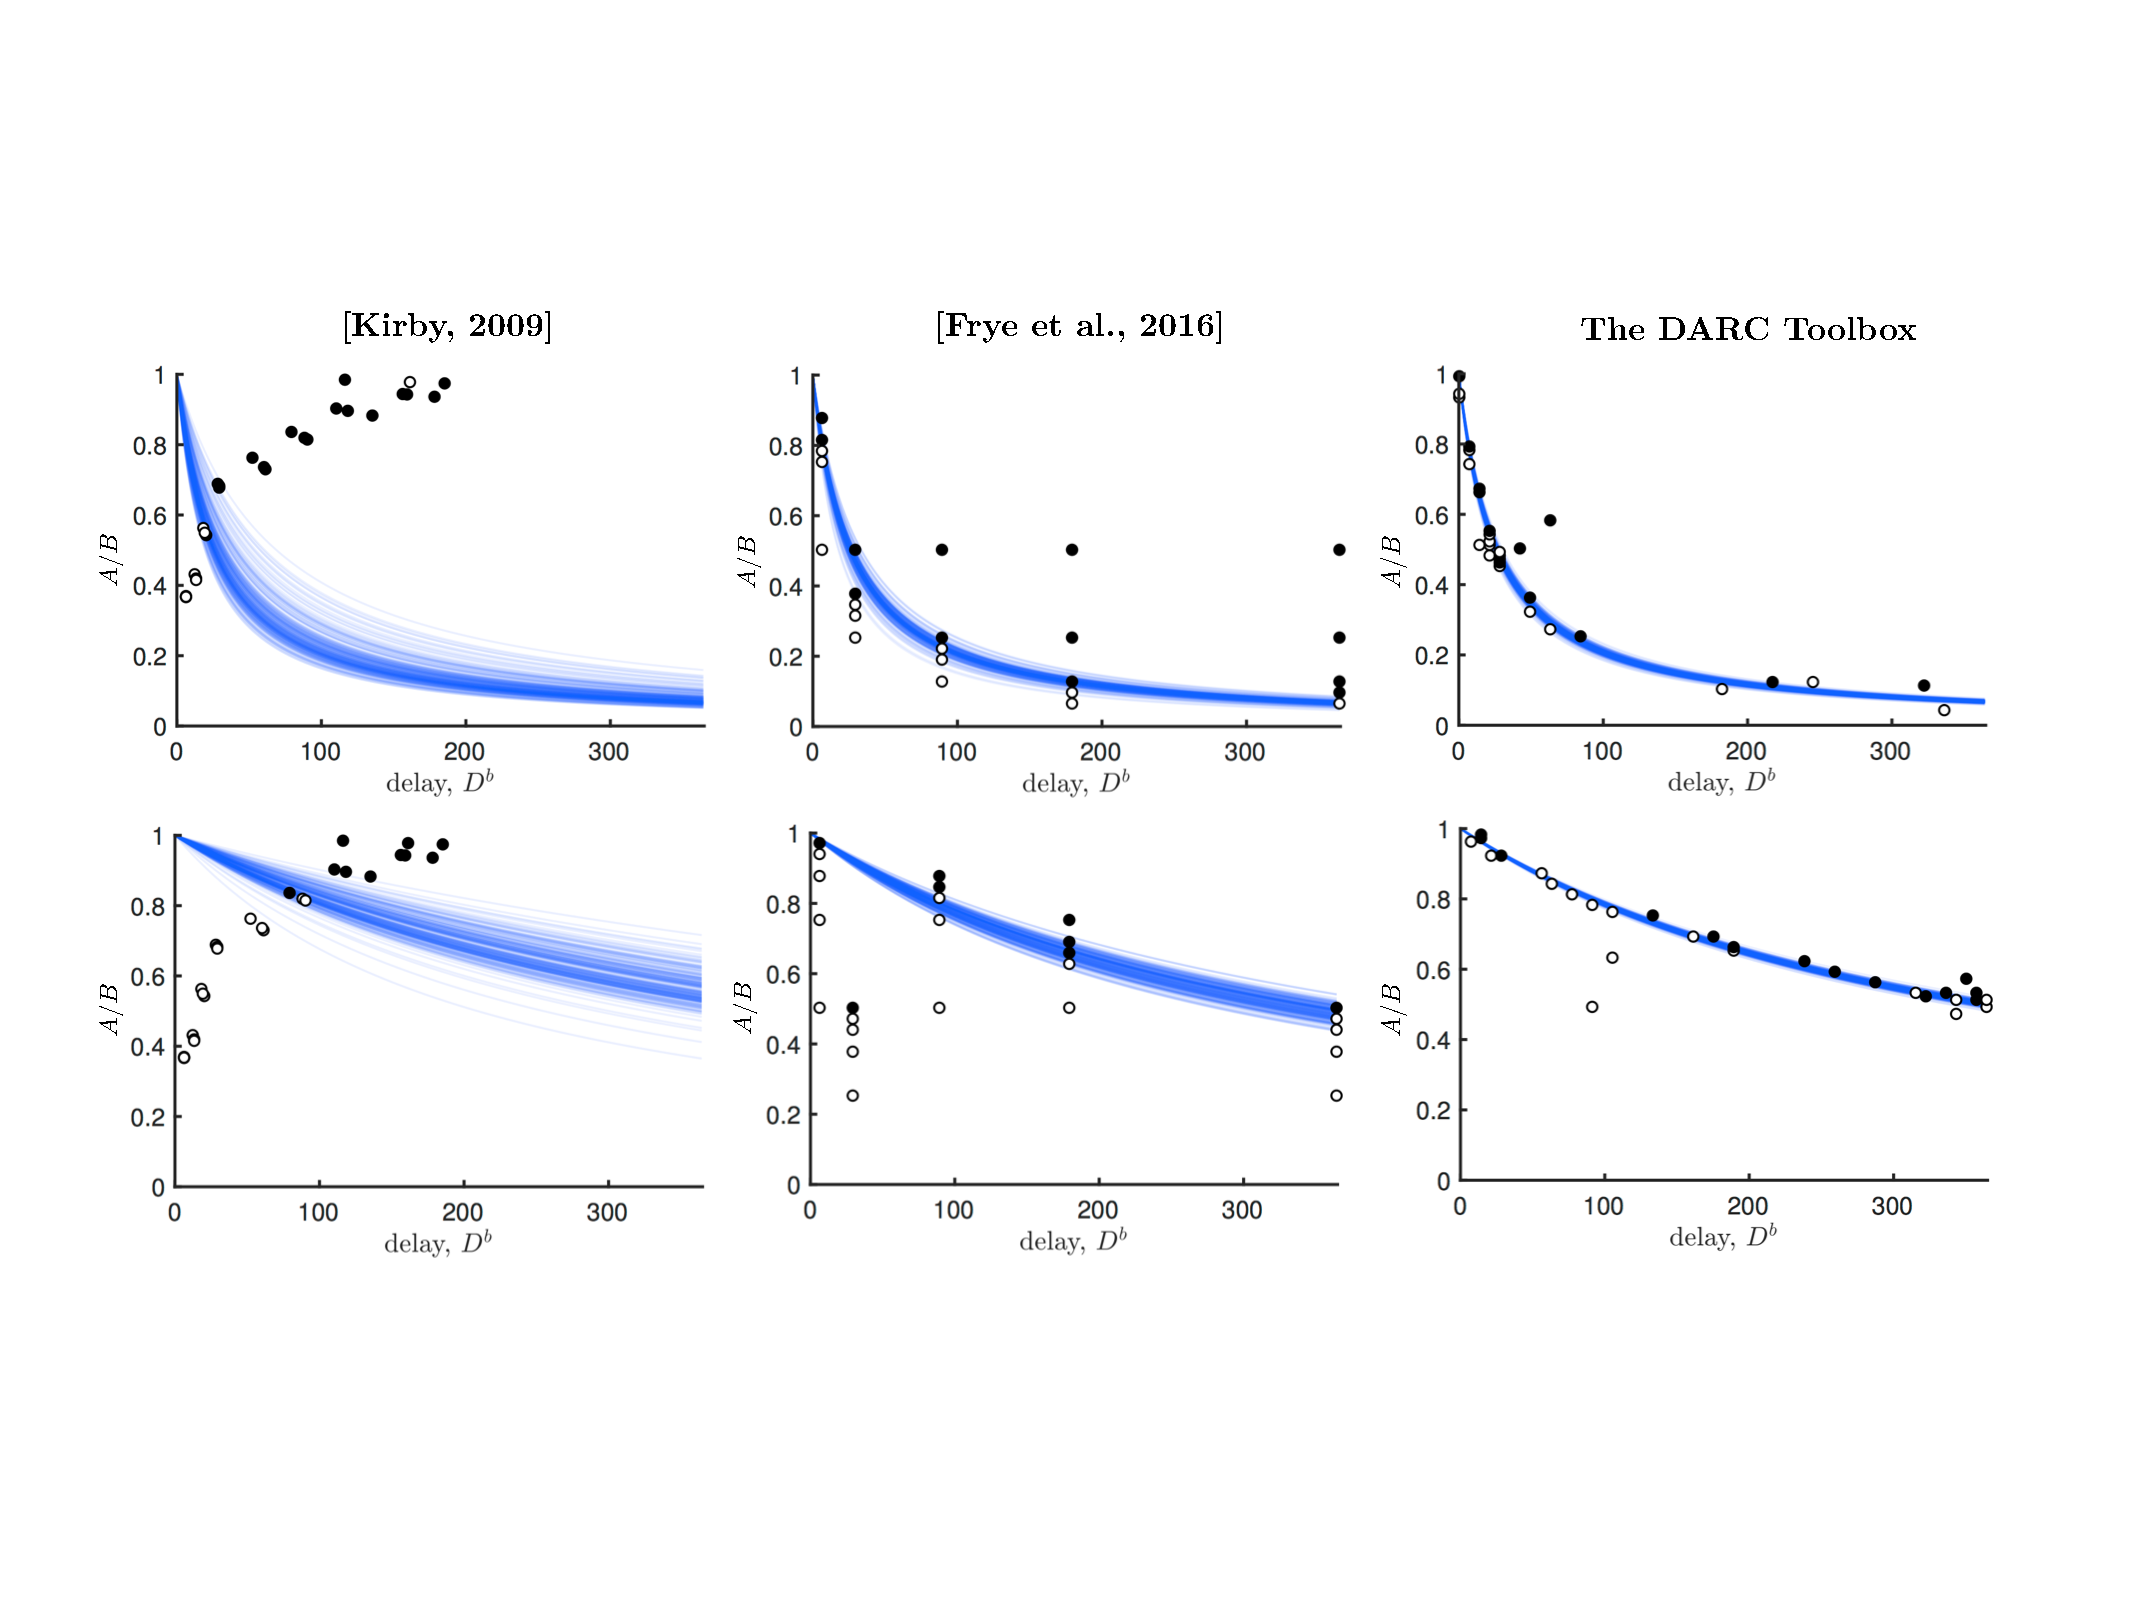
\includegraphics[width=\textwidth]{darc_results}
	\caption{Comparison of the DARC toolbox to alternative methods for two behavior styles: major
		depressive disorder (top) which indicates a relatively strong desire for immediate rewards ($k=0.04$)
		and anorexia nervosa (bottom) which indicates relatively low discounting rate ($k=0.0028$).  Lines show
		posterior samples from the final learned predictive distribution for the indifference curve (i.e. the curve
		along which the participant is equally likely to choose the immediate or dealy reward), circles represent
		questions where the delayed reward was preferred, and the filled dots correspond to the questions were
		the immediate reward was preferred.  The columns left to right corresponding to using the approaches
		of~\cite{Kirby:2009eu} which uses pre-fixed questions rather than using online adaptation,~\cite{Frye:2016eu}
		which uses a heuristic approach for choosing the best questions adaptively, and using our DARC toolbox
		which chooses questions using our sequential BED approach.  See~\cite{vincent2017darc} for further details.
		\label{fig:design:darc}
	}
\end{figure}

Finally, we examine the performance of the DARC toolbox compared to alternatives in the
psychology literature~\citep{Kirby:2009eu,Frye:2016eu} as shown in Figure~\ref{fig:design:darc}.  Using the
same likelihood model as~\eqref{eq:design:darc},
we fix $\alpha=2$ and set the prior on $k$ as $\log k \sim \mathcal{N}(-4.5,0.5^2)$.  We fixed $B=100$ and
then use three different methods for sequentially selecting designs $d_t = \{A_t,D^b_t\}$, for
two different hypothetical participants with respective ground truth parameters of $k=0.04$ and $k=0.0028$.
Responses are generated presuming the likelihood model is correct and sampling directly from
\eqref{eq:design:darc} using the ground truth parameters.  We then plot a characterization of the posterior
predictive after $27$ questions have been asked.  All methods are capable of working in real time, taking
about a second or less to choose the design at each iteration when run on a mid-range laptop.  Though 
hardly a rigorous performance assessment, these results are still demonstrative of the potential utility of our
method.  The non-adaptive scheme of~\cite{Kirby:2009eu} always asks the same questions regardless of
the participant's responses.  The heuristic method of~\cite{Frye:2016eu} does better, but is still somewhat
wasteful.  The DARC toolbox on the other hand, takes only a couple of questions before achieving a
reasonable representation of the response surface, such that almost all of the questions asked are clearly
pertinent and the final posterior predictive distribution has far lower entropy than the other approaches.